
\chapter*{Datos de la Asignatura}
\label{chap:00.datos.de.IyA}
  \addcontentsline{toc}{chapter}{Datos de la Asignatura}



  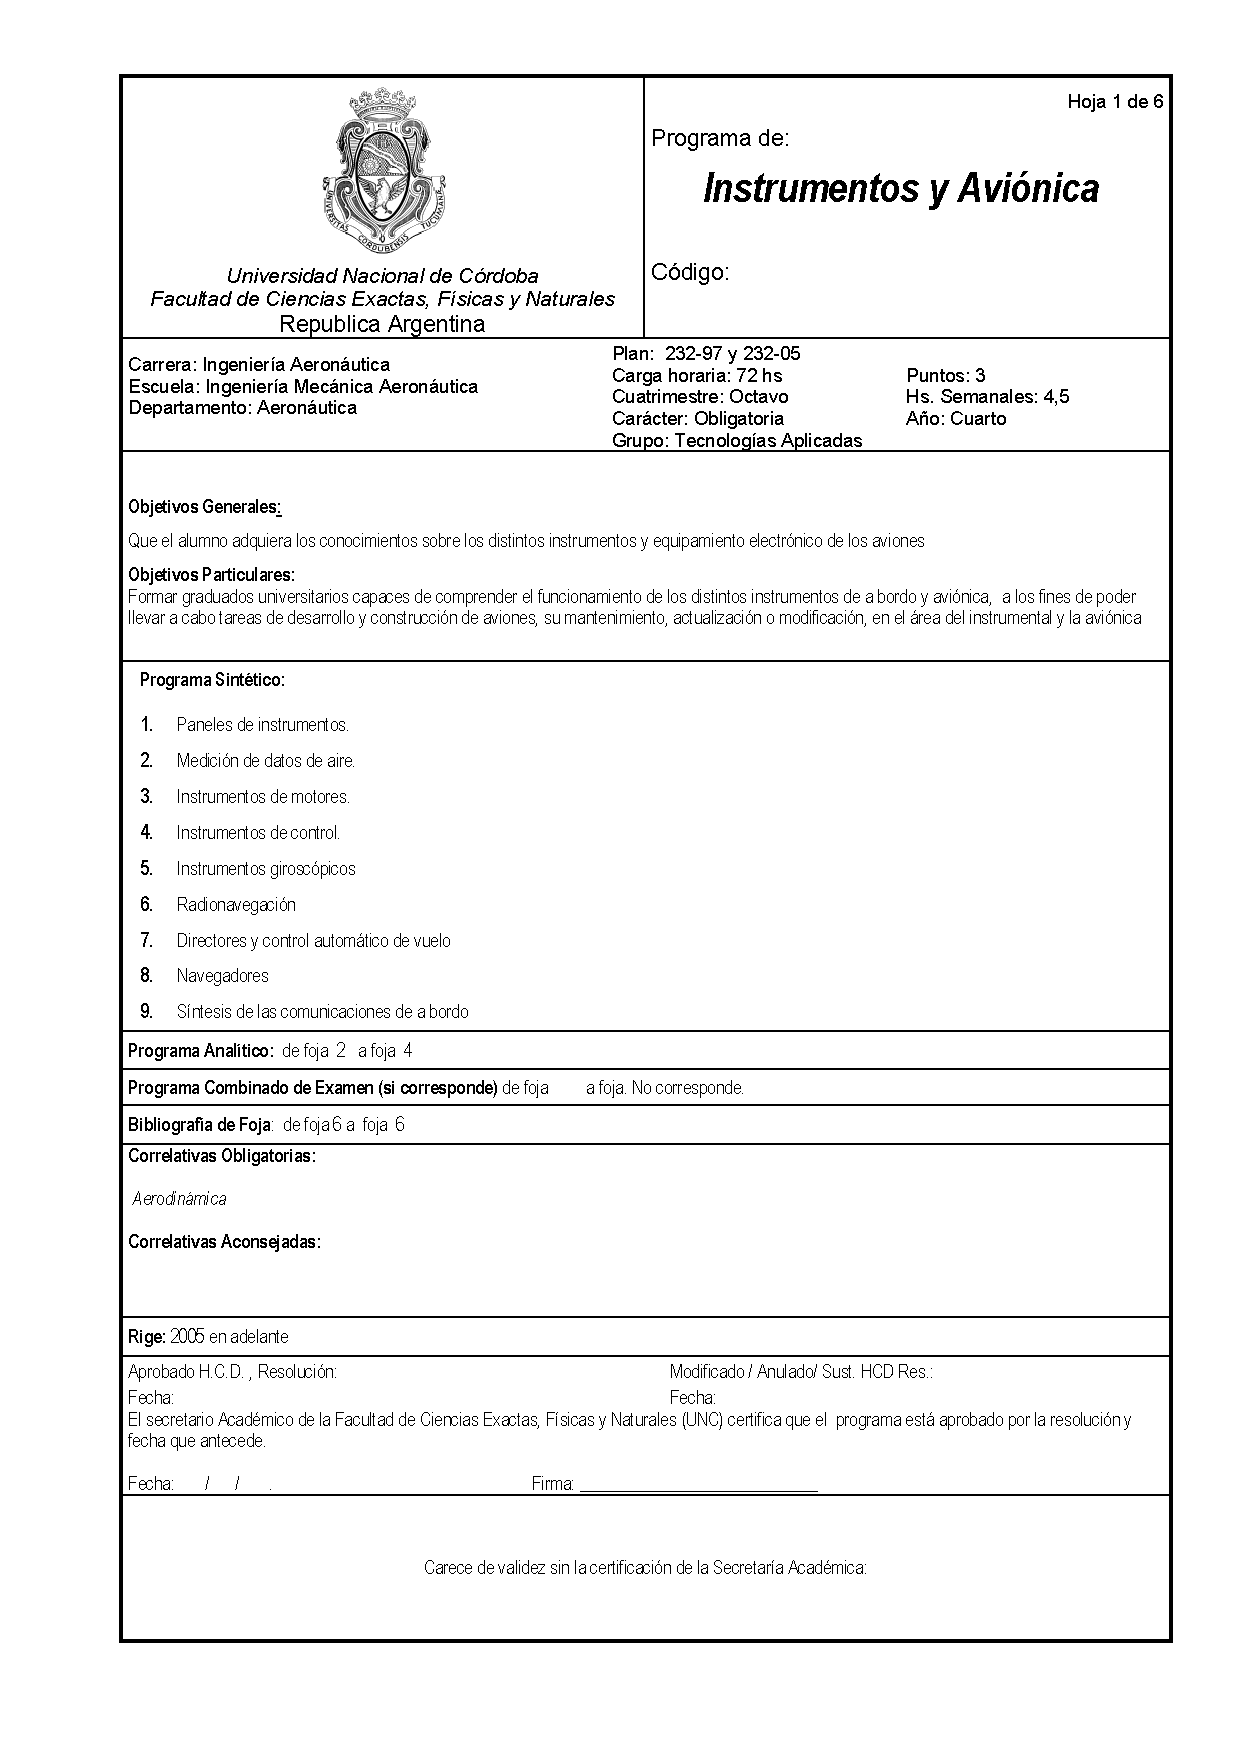
\includepdf[pages=-, fitpaper=false, scale=0.90, %landscape=true,
  offset = 0 -20,
  pagecommand={\thispagestyle{fancy}}]
  {00.Datos.IyA/Instrumentos_Y_Avionica.pdf}

\section*{Cronograma para el dictado de la Asignatura a\~no 2020}
\label{sec:00.cronograma}
  \addcontentsline{toc}{section}{Cronograma para el dictado a\~no 2020}

  \begin{itemize}
  \item Capítulo 1. Paneles de Instrumentos (García) 13/8/20
  \item Capítulo 2. Medición de datos de aire (Galeasso) 20/8/20
  \item Capítulo 3. Instrumentos de motores (Giraudo) 27/8/20
  \item Capítulo 4. Instrumentos de control (Giraudo) 3/9/20
  \item \textbf{Parcial 01 Todos, 10/9/2020 Abarca Capítulos 1 a 3}
  \item Capítulo 5. Instrumentos giroscópicos (Galeasso) 17/9/20
  \item Capítulo 6. Radionavegación (Garcia) 24/9/20
  \item Capítulo 7. Directores y control automático de vuelo ( García)     1/10/20
  \item Capítulo 8. Navegadores (Garcia) 8/10/20
  \item {\bf Parcial 02 Todos 15/10/2020 Abarca Capítulos 4 a 7}
  \item \textbf{Recuperatorios Todos 22/10/2020}
  \item Capítulo 8. Navegadores (GPS, nav. inerc.) (Giraudo) 29/10/20
  \item Capítulo 9. Síntesis de las comunicaciones de a bordo (Garcia)     5/11/20
  \item \textbf{Coloquio Todos 12/11/2020 Abarca todo el programa}
  \item \textbf{Coloquio Todos 19/11/2020 Abarca todo el programa}
  \end{itemize}


\section*{Docentes}
\label{00.docentes}
  \addcontentsline{toc}{section}{Docentes}

  \begin{tabular}{llm{0.5\textwidth}} \rowcolor{yellow!30}
 {\bf Docente} & {\bf Correo electr\'onico} & {\bf D\'ia, horario consulta, medio de consulta} \\ \rowcolor{cyan!20}
  Ing. Jorge Garcia & jgarcia@unc.edu.ar & D\'ia Mi\'ercoles, de 15 a 17 hs, correo electr\'onico, google meet \\ 
  Ing. Angel Galeasso & angel.galeasso@unc.edu.ar & D\'ia Mi\'ercoles, de 16 a 17 hs, correo electr\'onico, google meet    \\ \rowcolor{cyan!20} 
  Ing. Pedro Giraudo  & pedrogiraudo@unc.edu.ar &  D\'ia Mi\'ercoles, de 17:30 a 19 hs, correo electr\'onico, google meet, zoom     \\
\end{tabular}